\begin{example}
	\index{Example: Future event counts}
	\label{ex:events}
	Let $x=x_1+x_2+\dots x_M$ be the sum of future event counts and $y=\{y_1,y_2,y_3,\dots y_N\}$ be observed event counts. With this notation the expected\index{Expectation value} number of future events, $x$, and the associated uncertainty\index{Variance} can be written
	\begin{equation}
		\mathbb{E}[x|y,I]\pm \sqrt{\text{Var}[x|y,I]},
		\label{eq:mean_var}
	\end{equation}
	where
	\begin{equation}
		\begin{split}
			\mathbb{E}[x|y,I] &= \sum_i ip(x =i|y,I),\\
			\text{Var}[x|y,I] &=  \sum_i i^2p(x =i|y,I)-\mathbb{E}[x|y,I]^2.
		\end{split}
		\label{h1}
	\end{equation}
	The distribution over counts $p(x =i|y,I)$ can be expanded by marginalizing over a set of unknown parameters from underlying distributions. The details depend on the statistical assumptions imposed. In this example, different assumptions and their consequences will be investigated.
	
	\paragraph{Simple Poisson Assumption:} The most common assumption is to assume data follow a Poisson distribution\index{Poisson distribution} with an unknown rate parameter which will then be marginalized\index{Marginalized} over. An abvious choice of prior would be the conjugate gamma distribution\index{Gamma distribution} (which is also the distribution with maximum entropy\index{Maximum entropy}) with parameters $\alpha, \beta$, meaning
	\begin{equation}
		\begin{split}
			p(x =i|y,\alpha, \beta,I) &= \int d\lambda p(x =i,\lambda|y,\alpha, \beta,I)\\
			&=\int d\lambda p(x =i|\lambda,\alpha, \beta,y,I)p(\lambda|\alpha, \beta,y,I)\\
			&= \int d\lambda p(x =i|\lambda,\alpha, \beta,y,I)\frac{p(y|\lambda,\alpha, \beta,I)p(\lambda|\alpha, \beta,I)}{p(y|\alpha, \beta,I)}.
		\end{split}
		\label{h4}
	\end{equation}
	with
	\begin{equation}
		\begin{split}
			p(y|\alpha, \beta,I) & = \int d \lambda p(y|\alpha, \beta,\lambda,I)p(\lambda|\alpha, \beta,I),\\
			p(y|\alpha, \beta,\lambda,I) &= \prod_{j=1}^N\text{Poi}(y_j|\lambda)\\
			&= \lambda^{N\bar{y}}e^{-N\lambda}\prod_{j=1}^N \frac{1}{y_j!},\\
			p(\lambda|\alpha,\beta,I) &= \text{Ga}(\lambda|\alpha,\beta)\\ &=\frac{\beta ^\alpha}{\Gamma(\alpha)}\lambda^{\alpha-1}e^{-\beta \lambda}.
		\end{split}
	\end{equation}
	Meaning
	\begin{equation}
		p(y|\lambda,\alpha, \beta,I)p(\lambda|\alpha, \beta,I) = \frac{\beta^\alpha}{\Gamma(\alpha)}\lambda^{\alpha+N\bar{y}-1}e^{-(\beta+N)\lambda}\prod_{j=1}^N \frac{1}{y_j!}
	\end{equation}
	and consequently
	\begin{equation}
		\begin{split}
			\frac{p(y|\lambda,\alpha, \beta,I)p(\lambda|\alpha, \beta,I)}{p(y|\alpha, \beta,I)} &= \frac{\lambda^{\alpha+N\bar{y}-1}e^{-(\beta+N)\lambda}}{\int d\lambda \lambda^{\alpha+N\bar{y}-1}e^{-(\beta+N)\lambda}}\\
			&= \text{Ga}(\lambda|\alpha+N\bar{y},\beta+N)\\
		\end{split}
	\end{equation}
	Using that $p(x =i|\lambda,\alpha,\beta,y,I) = \text{Poi}(x =i|M\lambda)$ yields
	\begin{equation}
		\begin{split}
			\mathbb{E}[x|y,\alpha,\beta,I] &= \sum_ii\int d\lambda \text{Poi}(x = i|M\lambda)\text{Ga}(\lambda| \alpha+N\bar{y},\beta +N)\\
			&= M\int d\lambda\lambda\text{Ga}(\lambda | \alpha+N\bar{y},\beta +N)\\
			&= M \frac{\alpha+N\bar{y}}{\beta +N},
		\end{split}
	\end{equation}
	where for the second equality it has been used that $\sum_ii \text{Poi}(x = i|M\lambda)=M\lambda$ and for the second equality it has been realized that the second line denoted the expectation of a Gamma distribution with modified parameters. Similarly for the variance
	\begin{equation}
		\begin{split}
			\sum_i i^2p(x = i|y,\alpha,\beta,I) &=  \sum_ii^2\int d\lambda \text{Poi}(x =i|M\lambda)\text{Ga}(\lambda | \alpha+N\bar{y},\beta +N)\\
			&=M\int d\lambda (\lambda +M\lambda^2)\text{Ga}(\lambda|\alpha+N\bar{y},\beta +N)\\
			&=\mathbb{E}[x|y,\alpha,\beta,I]+M^2\int d\lambda \lambda^2\text{Ga}(\lambda|\alpha+N\bar{y},\beta +N)\\
			&=\mathbb{E}[x|y,\alpha,\beta,I]+M^2\frac{\alpha+N\bar{y}}{(\beta +N)^2}+\mathbb{E}[x|y,\alpha,\beta,I]^2\\
		\end{split}
		\label{h2}
	\end{equation}
	where for the second equality it has been used that $\sum_ii^2\text{Poi}(x = i|M\lambda)=\text{Var}[i|M\lambda]+\mathbb{E}[x|M\lambda]^2=M\lambda +M^2\lambda^2$ and similarly for the fourth equality. Combining equations \eqref{h1} and \eqref{h2}, the variance can be written
	\begin{equation}
		\begin{split}
			\text{Var}[x|y,\alpha,\beta,I] & = \mathbb{E}[x|y,\alpha,\beta,I]+M^2\frac{\alpha+N\bar{y}}{(\beta +N)^2}\\
			& = M\bigg(1+\frac{M}{\beta+N}\bigg)\frac{\alpha+N\bar{y}}{\beta +N}.\\
		\end{split}
	\end{equation}
	In the limit of $\beta,\alpha\rightarrow 0$ equation \eqref{eq:mean_var} become
	\begin{equation}
		\begin{split}
			\mathbb{E}[x|y,I]\pm \sqrt{\text{Var}[x|y,I]} & = \lim\limits_{\alpha,\beta\rightarrow 0}\big(\mathbb{E}[x|y,\alpha,\beta,I]\pm \sqrt{\text{Var}[x|y,\alpha,\beta,I]}\big)\\
			& = M\bar{y}\pm \sqrt{M\big(1+\frac{M}{N}\big)\bar{y}}.\\ 
		\end{split}
		\label{h3}
	\end{equation}
	Equation \eqref{h3} informs that the expected number of future events is equal to the mean number of observed events per day multiplied with the number of days -- That makes sense. The variance of equation \eqref{h3} is proportional to the square root of the observed mean event count, which is to be expected from a Poisson distribution. It means $\mathbb{E}[x|y,I]\gg \sqrt{\text{Var}[x|y,I]}$ for $\bar{y}\gg 1$ and hence that the uncertainty approaches a negligible quantity. This is a strong implicit statement which easily can be broken. This can for example happen if the number of events is expected to vary due to a rate parameter that changes every day due to underlying dynamics, e.g. weather conditions. 
	
	
	\paragraph{Advanced Poisson Assumption:} In the case where the rate parameter of the Poisson distribution\index{Poisson distribution} is expected to have significant time variance while retaining unimodality, it is more accurate to assume that each rate parameter is unique, but drawn from the same gamma distribution\index{Gamma distribution}, meaning
	\begin{equation}
		\begin{split}
			p(x = i|y,\xi,\zeta,I) &= \int d\{\lambda_x\}d\{\lambda_y\} d\alpha d\beta p(x = i,\{\lambda_x\},\{\lambda_y\} ,\alpha, \beta|y,\xi,\zeta,I)\\
			&=\int d\{\lambda_x\}d\{\lambda_y\}d\alpha d\beta p(x=i,\{\lambda_x\}|\alpha, \beta,y,\xi,\zeta,I)p(\{\lambda_y\},\alpha,\beta|y,\xi,\zeta,I),
		\end{split}
		\label{r1}
	\end{equation}
	where $\xi,\zeta$ are the parameters of the prior distributions, $d\{\lambda_x\} = d\lambda_{x_1}d\lambda_{x_2}\dots d\lambda_{x_M}$ and $d\{\lambda_y\}=d\lambda_{y_1}d\lambda_{y_2}\dots d\lambda_{y_N}$ and
	\begin{equation}
		\begin{split}
			p(x=i,\{\lambda_x\}|\alpha, \beta,y,\xi,\zeta,I) &= p(x=i|\{\lambda_x\},\alpha, \beta,y,I)p(\{\lambda_x\}|\alpha, \beta,I),\\
			p(\{\lambda_y\},\alpha,\beta|y,\xi,\zeta,I) & = \frac{p(y|\{\lambda_y\},\alpha, \beta,I)p(\{\lambda_y\}|\alpha, \beta,I)p(\alpha|\xi,I)p(\beta|\zeta,I)}{p(y|\xi,\zeta,I)}
		\end{split}
	\end{equation}
	with
	\begin{equation}
		\begin{split}
			p(y|\xi,\zeta,I) & = \int d\{\lambda_y\} d\alpha d\beta p(y|\{\lambda_y\},\alpha, \beta,I)p(\{\lambda_y\}|\alpha, \beta,I)p(\alpha|\xi,I)p(\beta|\zeta,I),\\
			p(y|\{\lambda_y\},\alpha, \beta,I)p(\{\lambda_y\}|\alpha, \beta,I) &= \prod_{j=1}^N\text{Poi}(y_j|\lambda_{y_j})\text{Ga}(\lambda_{y_j}|\alpha,\beta).\\
		\end{split}
	\end{equation}
	The integrals over gamma can be evaluated individually viz
	\begin{equation}
		\begin{split}
			p(y_i|\alpha,\beta,I) &= \int d \lambda_{y_i} \text{Poi}(y_j|\lambda_{y_j})\text{Ga}(\lambda_{y_j}|\alpha,\beta)\\
			& = \begin{pmatrix}
				y_j+\alpha-1\\
				y_j
			\end{pmatrix}
			\bigg(\frac{\beta}{\beta+1}\bigg)^{y_j}\bigg(\frac{1}{\beta +1}\bigg)^\alpha\\
			&= \text{NB}\bigg(y_j|\alpha,\frac{\beta}{\beta +1}\bigg),
		\end{split}
	\end{equation}
	where NB abbreviates the negative binomial distribution\index{Negative binomial distribution}. The sum of negative binomial random variables is another negative binomial random variable, such that
	\begin{equation}
		\int d\{\lambda_x\} p(x=i,\{\lambda_x\}|\alpha, \beta,y,I) = \text{NB}\bigg(x=i|M\alpha,\frac{\beta}{\beta +1}\bigg),
	\end{equation}
	meaning equation \eqref{r1} can be written
	\begin{equation}
		\begin{split}
			p(x = i|y,\xi,\zeta,I) &= \frac{1}{p(y|\xi,\zeta,I)}\int d\alpha d\beta \text{NB}\bigg(x=i|M\alpha,\frac{\beta}{\beta +1}\bigg)\prod_{j=1}^N\text{NB}\bigg(y_j|\alpha,\frac{\beta}{\beta +1}\bigg)p(\alpha|\xi,I)p(\beta|\zeta,I).
		\end{split}
		\label{r2}
	\end{equation}
	Using the principle of maximum\index{Maximum entropy}, entropy, the distributions for $\alpha$ and $\beta$ can be assigned gamma distributions
	\begin{equation}
		\begin{split}
			p(\alpha|\xi,I) & = p(\alpha|a,b,I)\\
			&= \text{Ga}(\alpha| a, b),\\
			p(\beta|\zeta,I) & = p(\beta|c,d,I)\\
			&= \text{Ga}(\alpha| c, d),\\
		\end{split}
	\end{equation}
	with $\xi = \{a,b\}$ and $\zeta = \{c,d\}$. With this setup, $\mathbb{E}[x|y,\xi,\zeta,I]\pm \sqrt{\text{Var}[x|y,\xi,\zeta,I]}$ can be evaluated numerically using numerical methods like e.g. Hamiltonian Monte Carlo (see appendix \ref{app:HMC}). In this example, the pymc python packge~\citep{pymc} will be used (which utilize Hamiltonian Monte Carlo) with parameters $a=b=c=d =1$, corresponding to wide (low bias) gamma distributions. 
	
	\paragraph{Normal Assumption:} In case the distribution of $x$ is fairly symmetric around its peak and the summary statistics of equation \eqref{eq:mean_var} are the quantities of primary interest, a crude normal approximation can be made. For a continuous variable, equation \eqref{h1} become		
	\begin{equation}
		\begin{split}
			\mathbb{E}[x|y,I] &= \int xp(x|y,I),\\
			\text{Var}[x|y,I] &=  \int x^2p(x|y,I)-\mathbb{E}[x|y,I]^2.
		\end{split}
		\label{h1con}
	\end{equation}
	Assume $x$ is normally distributed\index{Normal distribution} with mean and precision $\mu\sim N(\mu|\text{mean}=\mu_0,\text{variance}=\frac{1}{c\tau})$ and $\tau\sim \text{Ga}(\tau|\alpha,\beta)$ following a normal and gamma distribution\index{Gamma distribution}, respectively. In this case
	\begin{equation}
		p(x|y,\mu_0,c,\alpha,\beta,I) = \int d\mu  d\tau p(x|\mu,\tau,y,I)\frac{p(y|\mu,\tau,I)p(\mu|\tau,\mu_0,c,I)p(\tau|\alpha,\beta,I)}{p(y|\mu_0,c,\alpha,\beta,I)}.
		\label{h6}
	\end{equation}
	With these assumptions, the likelihood is given by
	\begin{equation}
		\begin{split}
			p(y|\mu,\tau,I) &= \bigg(\frac{\tau}{2\pi}\bigg)^{\frac{N}{2}}\prod_{j=1}^{N}e^{-\frac{\tau}{2}(\mu-y_j)^2}\\
			&=\bigg(\frac{\tau}{2\pi}\bigg)^{\frac{N}{2}}e^{-\frac{\tau}{2}\sum_{j=1}^{N}(\mu-y_j)^2}\\
		\end{split}
	\end{equation}
	and the expectation can be written
	\begin{equation}
		\begin{split}
			\mathbb{E}[x|y,\mu_0,c,\alpha,\beta,I] &=\frac{M\beta^{\alpha}}{p(y|I)\Gamma(\alpha)}\int d\mu d\tau \mu \bigg(\frac{\tau}{2\pi}\bigg)^{\frac{N}{2}}e^{-\frac{\tau}{2}\sum_{j=1}^{N}(\mu-y_j)^2}\sqrt{\frac{c\tau}{2\pi}}e^{-\frac{c\tau}{2}(\mu-\mu_0)^2}\tau^{\alpha-1}e^{-\tau \beta}\\
			&=M\frac{Z_1}{Z_0},\\
		\end{split}
		\label{h11}
	\end{equation}
	with
	\begin{equation}
		\begin{split}
			Z_1&\equiv \int d\tau \tau^{\alpha-\frac{1}{2}+\frac{N}{2}}e^{-\tau \beta} \int d\mu \mu e^{-\frac{\tau}{2}\sum_{j=1}^{N}(\mu-y_j)^2-\frac{c\tau}{2}(\mu-\mu_0)^2},\\
			Z_0 &\equiv\int d\tau \tau^{\alpha-\frac{1}{2}+\frac{N}{2}}e^{-\tau \beta} \int d\mu e^{-\frac{\tau}{2}\sum_{j=1}^{N}(\mu-y_j)^2-\frac{c\tau}{2}(\mu-\mu_0)^2}.
		\end{split}
		\label{h9}
	\end{equation}
	For the identification of $Z_1$ and $Z_0$ it has been used that all constants cancel out due to $p(y|I)$. The exponents involving $\mu$ can be rewritten 
	\begin{equation}
		\begin{split}
			-\frac{\tau}{2}\sum_{j=1}^{N}(\mu-y_j)^2-\frac{c\tau}{2}(\mu-\mu_0)^2 &= -\frac{\tau}{2}\sum_{j=1}^{N}(\mu-\bar{y}+\bar{y}-y_j)^2-\frac{c\tau}{2}(\mu-\mu_0)^2\\
			&=-\frac{\tau}{2}\sum_{j=1}^{N}(\bar{y}-y_j)^2-\frac{N\tau(\mu-\bar{y})^2}{2}-\tau(\mu-\bar{y})\sum_{j=1}^{N}(\bar{y}-y_j)-\frac{c\tau}{2}(\mu-\mu_0)^2\\
			&=-\frac{\tau}{2}\sum_{j=1}^{N}(\bar{y}-y_j)^2-\frac{N\tau(\mu-\bar{y})^2}{2}-\frac{c\tau}{2}(\mu-\mu_0)^2\\
			&=-\frac{\tau}{2}\sum_{j=1}^{N}(\bar{y}-y_j)^2-\frac{\tau}{2}(N+c)\bigg[\bigg(\mu-\frac{c\mu_0+N\bar{y}}{N+c}\bigg)^2 +\frac{cN\tau(\bar{y}-\mu_0)^2}{(c+N)^2}\bigg].\\
		\end{split}
		\label{h7}
	\end{equation}
	Only the second term in equation \eqref{h7} depend on $\mu$, so
	\begin{equation}
		e^{-\beta\tau}e^{-\frac{\tau}{2}\sum_{j=1}^{N}(\mu-y_j)^2-\frac{c\tau}{2}(\mu-\mu_0)^2} = e^{-\beta_0\tau}e^{-\frac{\tau}{2}(N+c)(\mu-\frac{c\mu_0+N\bar{y}}{N+c})^2},
		\label{h8}
	\end{equation}	
	with 
	\begin{equation}
		\beta_0\equiv \beta+\frac{1}{2}\sum_{j=1}^{N}(\bar{y}-y_j)^2+\frac{cN(\bar{y}-\mu_0)^2}{2(c+N)}.
	\end{equation}
	Using equation \eqref{h8} equation \eqref{h9} can be written
	\begin{equation}
		\begin{split}
			Z_1 &= \int d\tau \tau^{\alpha_0-\frac{1}{2}}e^{-\tau\beta_0} \int d\mu \mu e^{-\frac{\tau}{2}(N+c)(\mu-\frac{c\mu_0+N\bar{y}}{N+c})^2}\\
			&=\sqrt{\frac{2\pi}{N+c}}\frac{c\mu_0+N\bar{y}}{N+c}\beta_0^{-\alpha_0}\Gamma(\alpha_0), \\ 
			Z_0 &= \int d\tau \tau^{\alpha_0-\frac{1}{2}}e^{-\tau\beta_0} \int d\mu e^{-\frac{\tau}{2}(N+c)(\mu-\frac{c\mu_0+N\bar{y}}{N+c})^2}\\
			&=\sqrt{\frac{2\pi}{N+c}}\beta_0^{-\alpha_0}\Gamma(\alpha_0)
		\end{split}
		\label{h10}
	\end{equation} 
	where $\alpha_0\equiv \alpha+\frac{N}{2}$. Combining equation \eqref{h11} with \eqref{h10} yields
	\begin{equation}
		\mathbb{E}[x|y,\mu_0,c,\alpha,\beta,I]= M\frac{c\mu_0+N\bar{y}}{c+N}
	\end{equation}
	For the variance
	\begin{equation}
		\begin{split}
			\mathbb{E}[x^2|y,\mu_0,c,\alpha,\beta,I] &= \int d\mu d\tau dx x^2p(x|\mu,\tau,y,I)\frac{p(y|\mu,\tau,I)p(\mu|\tau,\mu_0,c,I)p(\tau|\alpha,\beta,I)}{p(y|\mu_0,c,\alpha,\beta,I)}\\
			&=\frac{M}{p(y|\mu_0,c,\alpha,\beta,I)}\int d\mu d\tau (M\mu^2+\tau^{-1}) p(y|\mu,\tau,I)p(\mu|\tau,\mu_0,c,I)p(\tau|\alpha,\beta,I)\\
			&=M\frac{MZ_2+Z_3}{Z_0}
		\end{split}
		\label{h12}
	\end{equation}
	where
	\begin{equation}
		\begin{split}
			Z_2 &= \int d\tau \tau^{\alpha_0-\frac{1}{2}}e^{-\tau\beta_0} \int d\mu \mu^2 e^{-\frac{\tau}{2}(N+c)(\mu-\frac{c\mu_0+N\bar{y}}{N+c})^2}\\
			& = \sqrt{\frac{2\pi}{(N+c)}}\bigg[\frac{1}{N+c}\beta_0^{1-\alpha_0}\Gamma(\alpha_0-1)+\bigg(\frac{c\mu_0+N\bar{y}}{N+c}\bigg)^2\beta_0^{-\alpha_0}\Gamma(\alpha_0) \bigg],\\
			Z_3 &= \int d\tau \tau^{\alpha_0-\frac{3}{2}}e^{-\tau\beta_0} \int d\mu  e^{-\frac{\tau}{2}(N+c)(\mu-\frac{c\mu_0+N\bar{y}}{N+c})^2}\\
			&=\sqrt{\frac{2\pi}{(N+c)}}\beta_0^{1-\alpha_0}\Gamma(\alpha_0-1)
		\end{split}
		\label{h13}
	\end{equation}
	Combining equations \eqref{h1}, \eqref{h12} and \eqref{h13}
	\begin{equation}
		\text{Var}[x|y,\mu_0,c,\alpha,\beta,I]=M\bigg(\frac{M}{N+c}+1\bigg)\frac{\beta_0}{\alpha_0-1}
	\end{equation}
	In the limit of $\mu_0,c,\alpha,\beta\rightarrow 0$ then
	\begin{equation}
		\begin{split}
			\mathbb{E}[x|y,I]\pm \sqrt{\text{Var}[x|y,I]} &= \lim\limits_{\mu_0,c,\alpha,\beta\rightarrow 0}\big(\mathbb{E}[x|y,\mu_0,c,\alpha,\beta,I]\pm \sqrt{\text{Var}[x|y,\mu_0,c,\alpha,\beta,I]}\big)\\ 
			&= M\bar{y}\pm \sqrt{M\frac{N+M}{N}\frac{N-1}{N-2}}\delta y\\ 
		\end{split}
		\label{h14}
	\end{equation}
	where 
	\begin{equation}
		\delta y \equiv \sqrt{\frac{\sum_{j=1}^{N}(\bar{y}-y_j)^2}{N-1}}
	\end{equation}
	is the sample standard deviation. From equation \eqref{h14}, it is clear that the result is close to the sample mean with uncertainty close to the sample standard deviation.
	
	\paragraph{Numerical example and comparison of approximations: } In order to illustrate the difference between the approximations considered in this example, consider a numerical example where data is drawn from a Poisson distribution with a rate parameter that is drawn from a gamma distribution with parameters $\alpha = 10$ and $\beta =  0.01$. $300$ counts are drawn, yielding the data shown in figure \ref{fig:q1}. Given the data shown in figure \ref{fig:q1}, the three approximations return the posterior predicitve distributions ($M=1$) shown in figure \ref{fig:q2} with expectations and standard deviations shown in table \ref{tab:1}. From figure \ref{fig:q2} it is clear that the approximations yield significantly different distributions. From table \ref{tab:1} it is clear that the expectation values are highly similar, whereas the standard deviations differ significantly. The distributions underlying each approximation (Poisson, negative binomial and normal) are unimodal, and as such it is expected that they will estimate the expectation value of unimodal data accurately. The Poisson distribution has a standard deviation that is determined by the expectation value (see equation \eqref{h3}) and as such it cannot accurately describe the variance in data where the expectation and variance is decoupled. In the advanced Poisson approximation, the mean and variance are decoupled and hence an accurate description of data is seen. Relative to the advanced Poisson approximation, the normal approximation suffer from three shortcommings i) it assumes the discrete events are continuous, ii) it assumes the distribution is symmetric and iii) it allows the counts to be negative (see the left tail of figure \ref{fig:q2} (bottom)). In relation to the expectation and standard deviation neither of the shortcommings are highly significant, however, they may be if different questions are asked of the posterior predictive.	
	\begin{figure}[H]
		\centering
		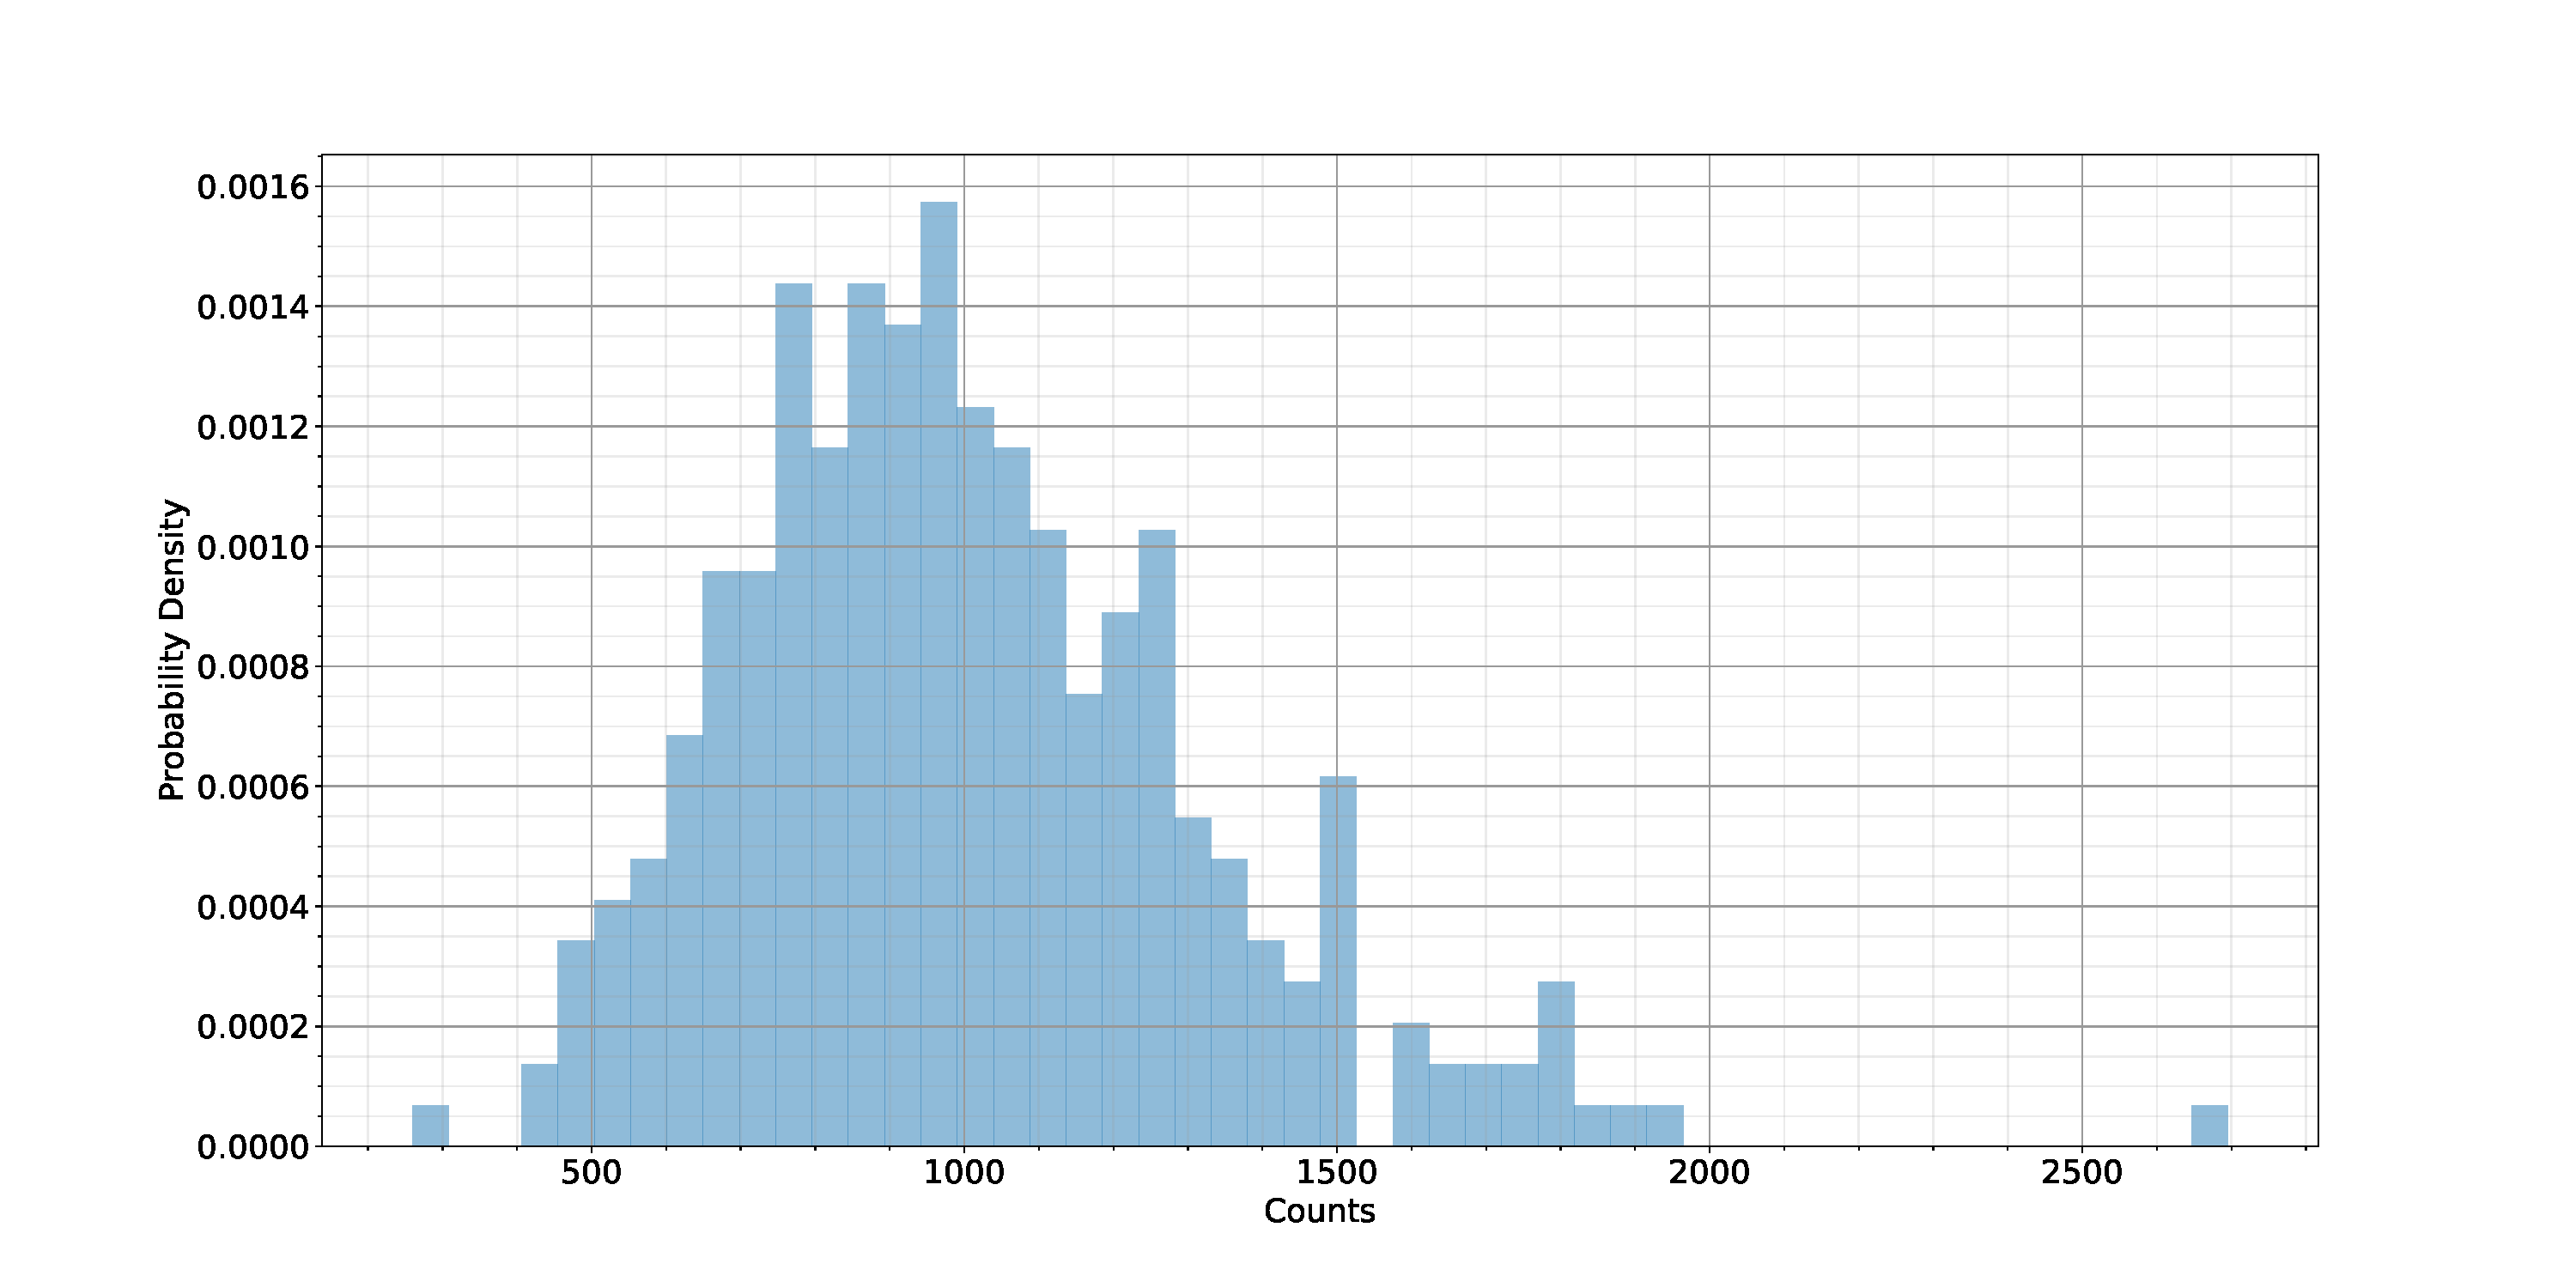
\includegraphics[width = 1\textwidth]{figures/count_hist.pdf}
		\caption{A probability density histogram for the sample of $300$ data points considered in the numerical example. The data are event counts drawn from ($300$) Poisson distributions with ($300$) rate parameters drawn from a gamma distribution with $\alpha = 10$ and $\beta =  0.01$.}
		\label{fig:q1}
	\end{figure}
	
	\begin{table}[h]
		\centering
		\begin{tabular}{|c|c|c|}
			\hline
			\multicolumn{1}{|c|}{Approximation} & \multicolumn{1}{c|}{$\mathbb{E}[x|y,I]$} & \multicolumn{1}{c|}{$\sqrt{\text{Var}[x|y,I]}$} \\
			\hline\hline
			Simple Poisson theoretical & $1008.9$ & $31.8$ \\
			Simple Poisson pymc & $1008.5$ & $31.8$ \\
			\hline
			Advanced Poisson pymc & $1008.7$ & $324.1$ \\
			\hline
			Normal theoretical & $1008.9$ & $321.3$\\
			Normal pymc & $1007.5$ & $322.2$\\
			\hline
		\end{tabular}
		\caption{Equation \eqref{eq:mean_var} computed by each of the three approximations considered here.}
		\label{tab:1}
	\end{table}
	
	\begin{figure}[H]
		\centering
		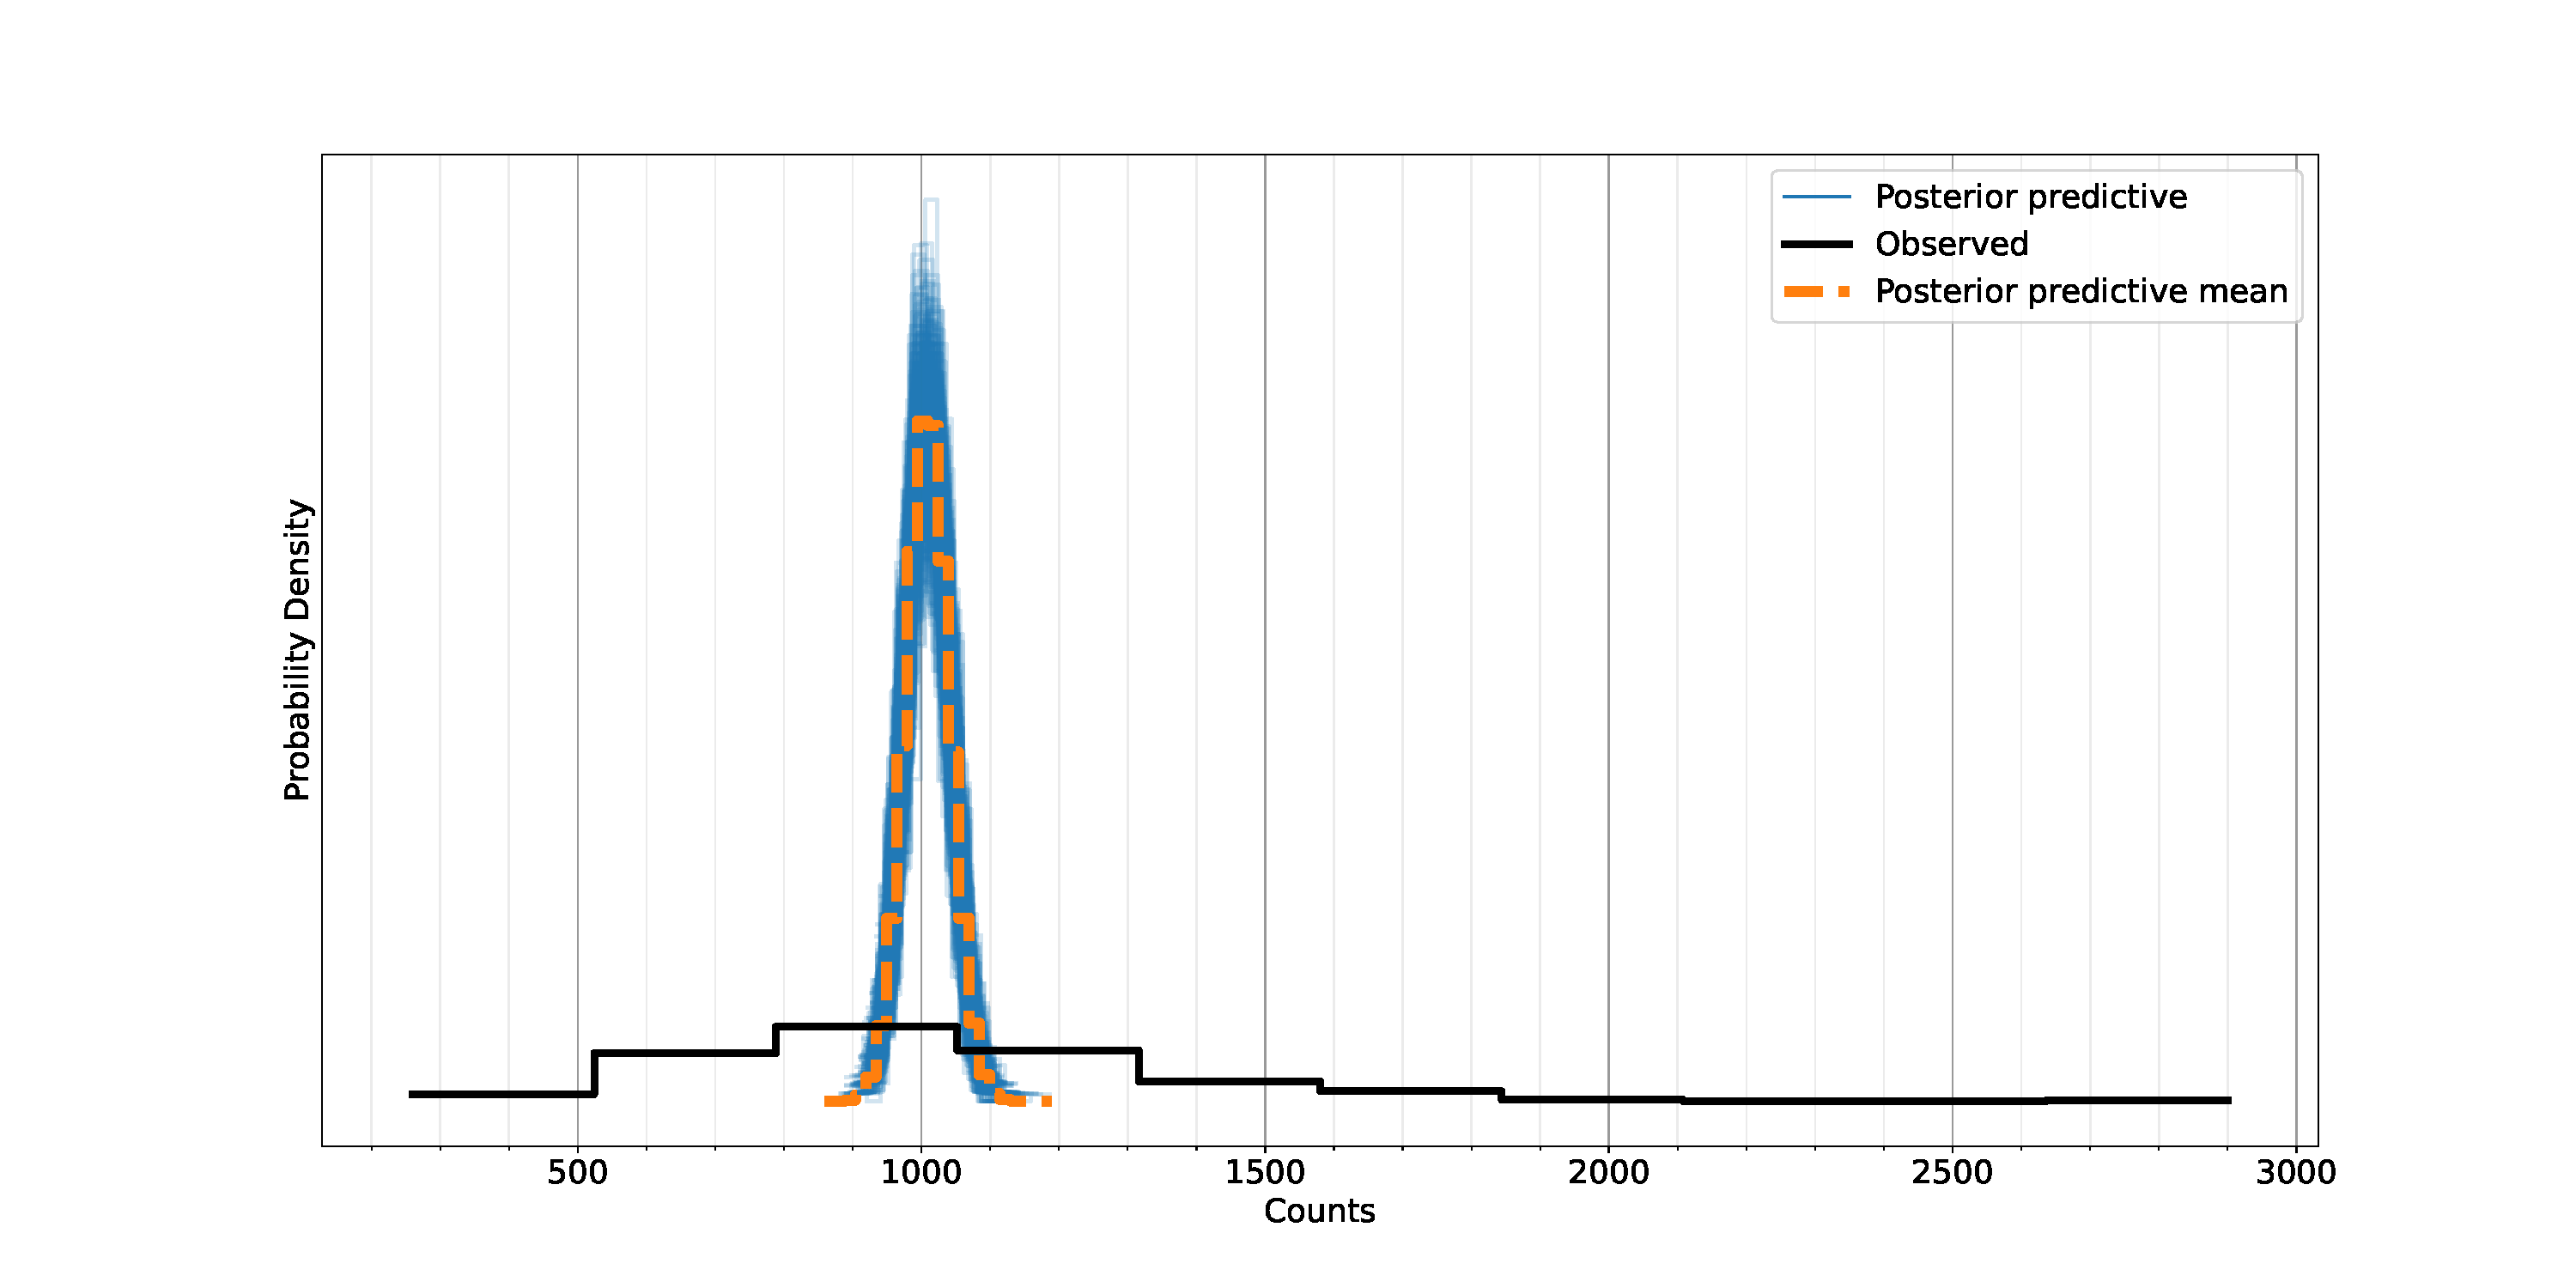
\includegraphics[width = 0.8\textwidth]{figures/pymc_poisson.pdf}
		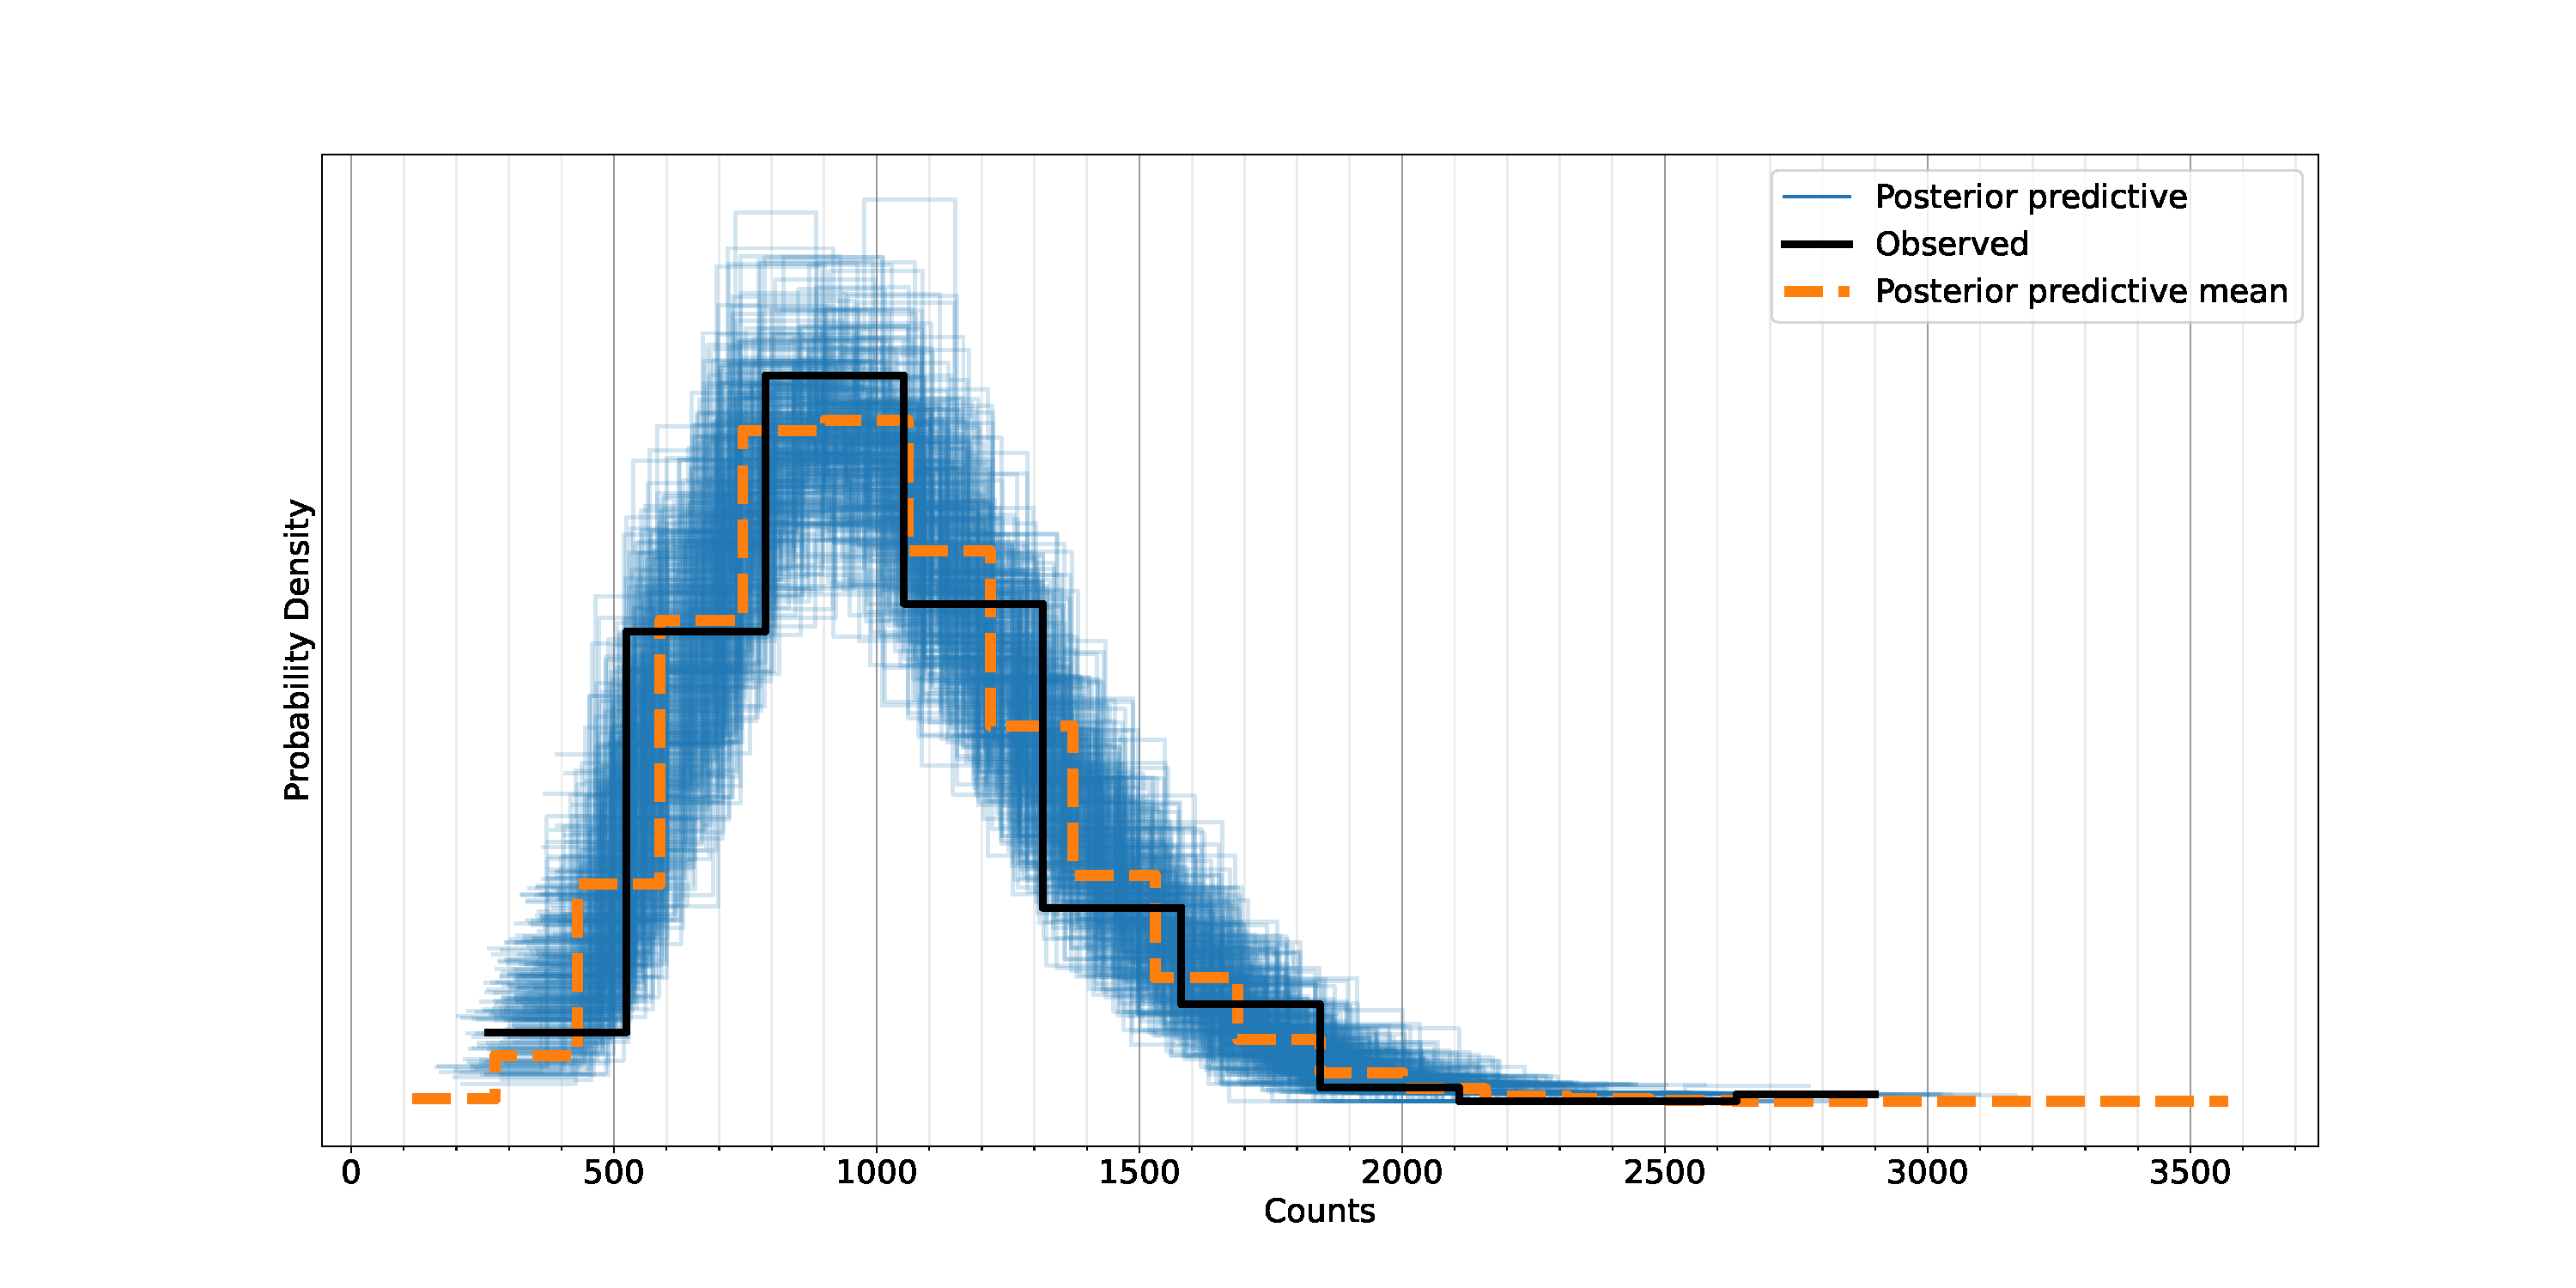
\includegraphics[width = 0.8\textwidth]{figures/pymc_negbin.pdf}
		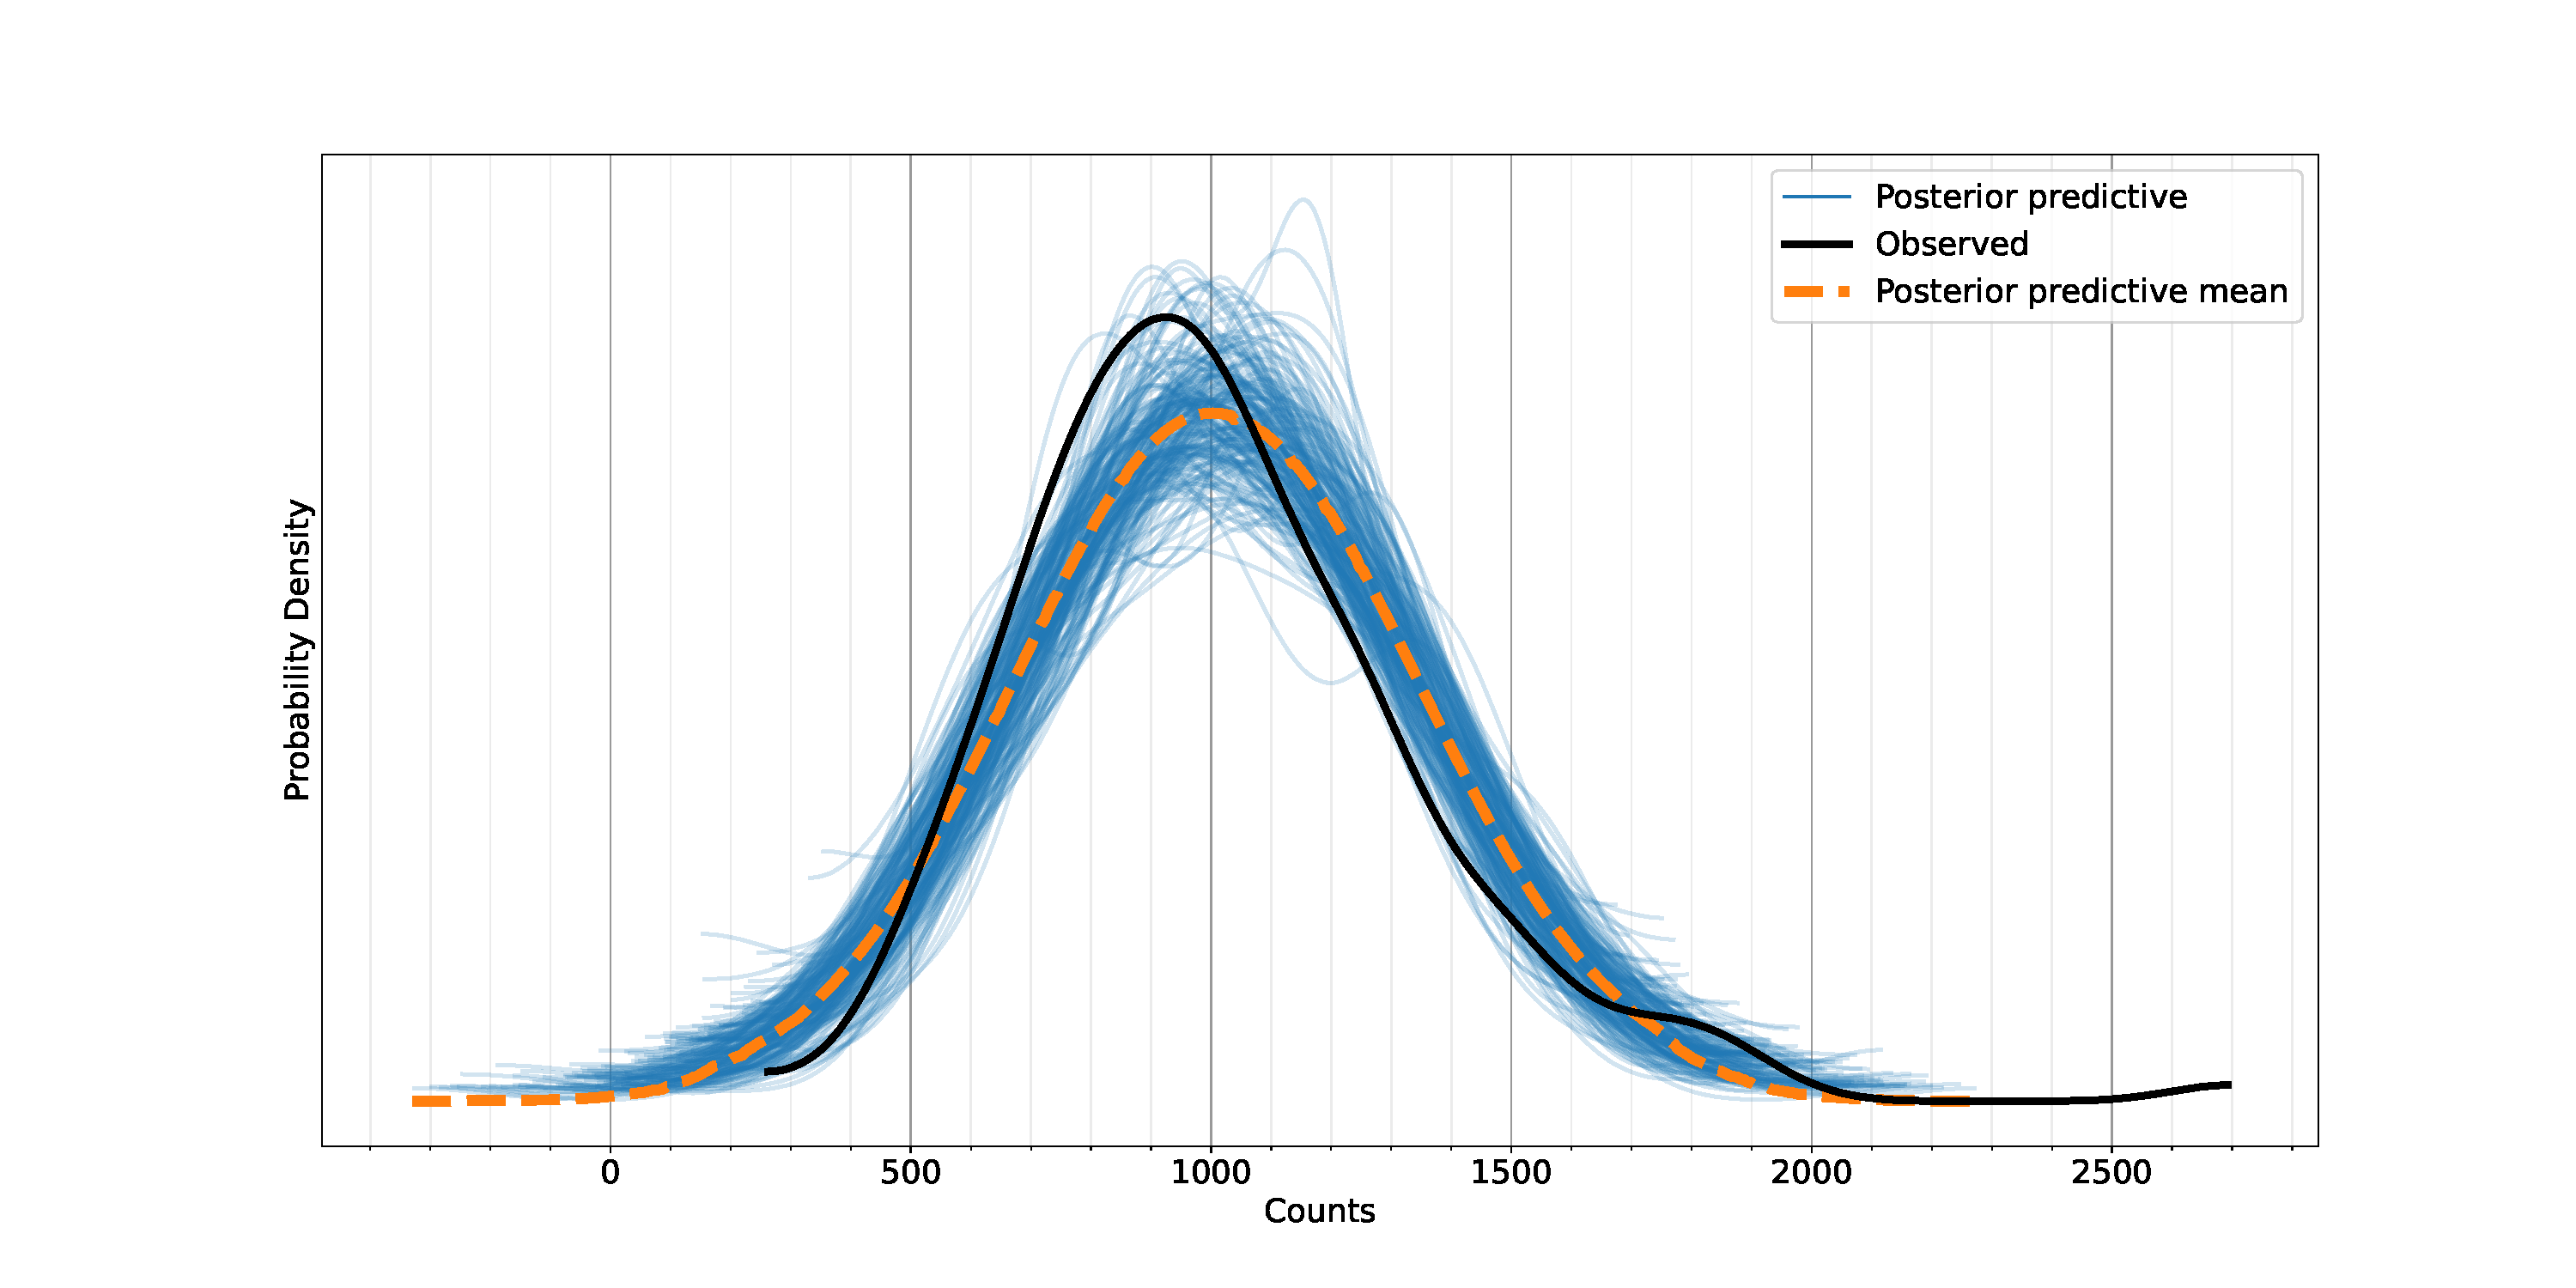
\includegraphics[width = 0.8\textwidth]{figures/pymc_normal.pdf}
		\caption{The posterior predictive distributions for the numerical example for each approximation. (top) is the simple Poisson approximation, (middle) is the advanced Poisson approximation and (bottom) is the normal approximation.}
		\label{fig:q2}
	\end{figure}
	
\end{example}